\documentclass[border=6pt]{standalone}
\usepackage{tikz}
\usetikzlibrary{
  arrows.meta,   % mũi tên Stealth, Latex, …
  calc,          % tính toán toạ độ
  positioning    % định vị node
}

% Thiết lập mặc định cho TikZ
\tikzset{
  >=Stealth,                % mũi tên Stealth
  line cap=round,
  line join=round
}

\begin{document}
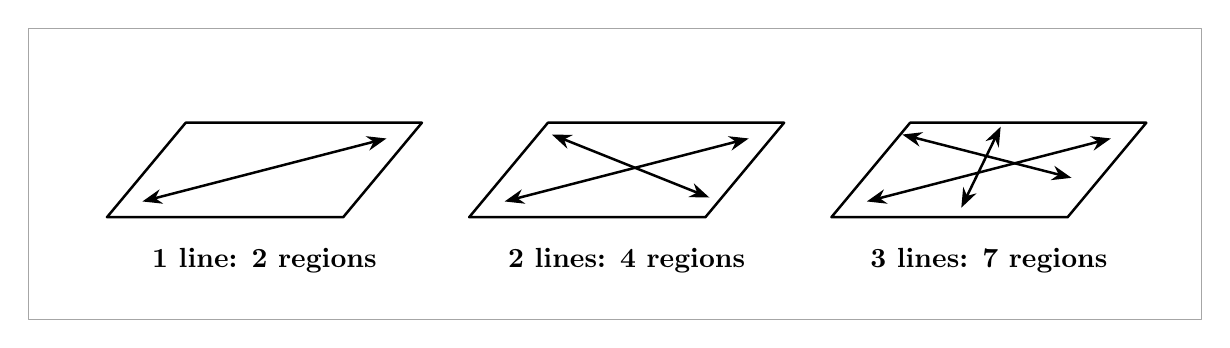
\begin{tikzpicture}[line cap=round,line join=round,>=Stealth]
  % --- overall frame (as in the screenshot) ---
  \draw[gray!70] (-0.7,-1.1) rectangle (14.2,2.6);

  % Common style
  \tikzset{
    pane/.style={line width=.9pt},
    cut/.style={line width=.9pt,<->}
  }

  % ========== (1) ==========
  \begin{scope}[shift={(0.3,0.2)}]
    % parallelogram
    \draw[pane] (0,0) -- (3,0) -- (4,1.2) -- (1,1.2) -- cycle;
    % 1 line
    \draw[cut] (0.45,0.20) -- (3.55,1.00);
    % label
    \node[font=\bfseries] at (2,-0.55) {1 line: 2 regions};
  \end{scope}

  % ========== (2) ==========
  \begin{scope}[shift={(4.9,0.2)}]
    % parallelogram
    \draw[pane] (0,0) -- (3,0) -- (4,1.2) -- (1,1.2) -- cycle;
    % 2 lines
    \draw[cut] (0.45,0.20) -- (3.55,1.00);
    \draw[cut] (1.05,1.05) -- (3.05,0.25);
    % label
    \node[font=\bfseries] at (2,-0.55) {2 lines: 4 regions};
  \end{scope}

  % ========== (3) ==========
  \begin{scope}[shift={(9.5,0.2)}]
    % parallelogram
    \draw[pane] (0,0) -- (3,0) -- (4,1.2) -- (1,1.2) -- cycle;
    % 3 lines
    \draw[cut] (0.45,0.20) -- (3.55,1.00);
    \draw[cut] (0.90,1.05) -- (3.05,0.5);
    \draw[cut] (1.65,0.12) -- (2.15,1.15);
    % label
    \node[font=\bfseries] at (2,-0.55) {3 lines: 7 regions};
  \end{scope}
\end{tikzpicture}

\end{document}